\section{Übung - PL/SQL}
\label{sec:uebung_02}
Führe den Inhalt des Skripts oehr\_dwhSS18.sql aus dem Verzeichnis data aus. Dadurch wird in Ihrer Umgebung eine reduzierte Version des DWH-Schemas bereitgestellt.

% ##########################################################################
% ############################### Aufgabe 01 ###############################
% ##########################################################################
\subsection{Aufgabe}
\label{subsec:uebung_02.aufgabe_01}
Schreiben Sie eine Prozedur, welche auf die Tabelle LOCATIONS zugreift und
\begin{itemize}
  \item den Inhalt in einer Nested Table ablegt,
  \item die ersten 12 Zeilen, geordnet nach LOCATION\_ID, in ein Varray legt,
  \item die CITY, referenziert durch die LOCATION\_ID, in einem Assoziativen Array ablegt.
\end{itemize}
Anschließend sollen die LOCATION\_ID und CITY aller drei Collections ausgegeben werden.

\subsubsection*{Lösung}
\label{subsubsec:uebung_02.aufgabe_01.loesung}
\inputsql{./loesungen/uebung_02/uebung_02_-_aufgabe_01.sql}


% ##########################################################################
% ############################### Aufgabe 02 ###############################
% ##########################################################################
\subsection{Aufgabe}
\label{subsec:uebung_02.aufgabe_02}
Schreiben Sie eine Table Function, der eine CHANNEL\_CLASS\_ID übergeben wird und für diese Absatzklasse die Bezeichnung, Absatzkanäle, die Anzahl aller Bestellungen sowie den durchschnittlichen Bestellwert über den Absatzkanal in einer Collection zurückgibt.

Bei Aufruf der Funktion könnte die Ausgabe für die CHANNEL\_CLASS\_ID = 13 wie folgt aussehen:

\begin{figure}[H]
  \centering
  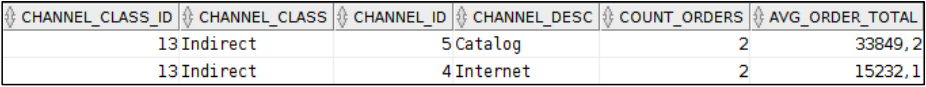
\includegraphics[width=0.85\textwidth]{img//uebung_02_-_aufgabe_02.png}
  \label{img:uebung_02_-_aufgabe_02}
  \caption{Table Function}{CHANNEL\_CLASS\_ID = 13}
\end{figure} 


\subsubsection*{Lösung}
\label{subsubsec:uebung_02.aufgabe_02.loesung}
\inputsql{./loesungen/uebung_02/uebung_02_-_aufgabe_02.sql}


% ##########################################################################
% ############################### Aufgabe 03 ###############################
% ##########################################################################
\subsection{Aufgabe}
\label{subsec:uebung_02.aufgabe_03}
Schreiben Sie eine Table Function, der eine Referenz auf einen Cursor übergeben wird. Dieser soll Kundendatensätze beinhalten und es soll für jeden übergebenen Datensatz der Name des Kunden, sein Land und der durch ihn generierte Umsatz in einer Collection zurückgegeben werden.

Ein exemplarischer Aufruf der Funktion könnte dabei wie folgt aussehen:
\begin{minted}[linenos, autogobble, breaklines,]{sql}
SELECT *
FROM TABLE(
  tf_customer(
    CURSOR(
      SELECT *
      FROM customers
      WHERE customer_id < 200
    )
  )
);
\end{minted}

Rückgabe bei Aufruf der Table Funktion:
\begin{figure}[H]
  \centering
  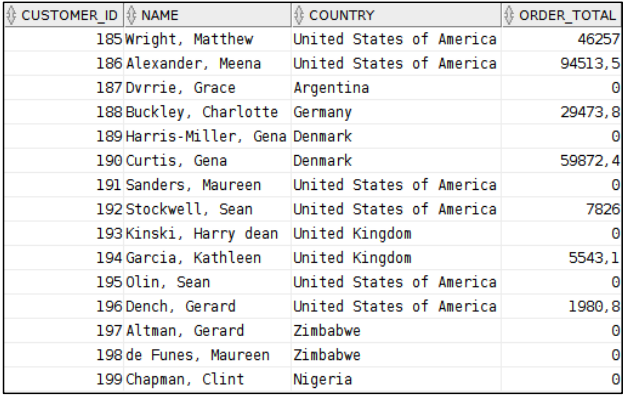
\includegraphics[width=0.75\textwidth]{img//uebung_02_-_aufgabe_03.png}
  \label{img:uebung_02_-_aufgabe_03}
  \caption{Rückgabe}{Rückgabe bei Aufruf der Table Function}
\end{figure} 

\subsubsection*{Lösung}
\label{subsubsec:uebung_02.aufgabe_03.loesung}
\inputsql{./loesungen/uebung_02/uebung_02_-_aufgabe_03.sql}


% ##########################################################################
% ############################### Aufgabe 04 ###############################
% ##########################################################################
\subsection{Aufgabe}
\label{subsec:uebung_02.aufgabe_04}
Ändern Sie die Funktion aus Aufgabe \ref{subsec:uebung_02.aufgabe_03} so ab, dass es sich um eine Pipelined Table Function handelt.

\subsubsection*{Lösung}
\label{subsubsec:uebung_02.aufgabe_04.loesung}
\inputsql{./loesungen/uebung_02/uebung_02_-_aufgabe_04.sql}


% ##########################################################################
% ############################### Aufgabe 05 ###############################
% ##########################################################################
\subsection{Aufgabe}
\label{subsec:uebung_02.aufgabe_05}
Schreiben Sie eine Prozedur, die für jede Tabelle in Ihrem Schema eine Kopie mit dem Präfix „tmp\_“ anlegt.

Hinweis: Die View USER\_TABLES listet alle eigenen Tabellen und eine Tabellenkopie kann mit folgendem DDL-Statement erzeugt werden:
\begin{minted}[linenos, autogobble, breaklines,]{sql}
CREATE TABLE tmp_tabname AS
  SELECT *
  FROM tabname;
\end{minted}

\subsubsection*{Lösung}
\label{subsubsec:uebung_02.aufgabe_05.loesung}
\inputsql{./loesungen/uebung_02/uebung_02_-_aufgabe_05.sql}


% ##########################################################################
% ############################### Aufgabe 06 ###############################
% ##########################################################################
\subsection{Aufgabe}
\label{subsec:uebung_02.aufgabe_06}
Erzeugen Sie eine weitere Prozedur, die ein Pattern (z.B. '\%A\%') über einen Eingabeparameter erwartet und alle Tabellen löscht, deren Name dem übergebenen Pattern entspricht. Verwenden Sie BIND Variablen wo es möglich ist.

\subsubsection*{Lösung}
\label{subsubsec:uebung_02.aufgabe_06.loesung}
\inputsql{./loesungen/uebung_02/uebung_02_-_aufgabe_06.sql}
